\documentclass{beamer}
\usetheme{Copenhagen}
\setbeamertemplate{headline}{}
\addtobeamertemplate{navigation symbols}{}{%
    \usebeamerfont{footline}%
    \usebeamercolor[fg]{footline}%
    \hspace{1em}%
    \insertframenumber/\inserttotalframenumber
}
\usepackage{amsmath,amsfonts,amssymb}
\usepackage[utf8]{vietnam}
\AtBeginDocument{
  \renewcommand{\figurename}{Figure}
  \renewcommand{\tablename}{Table}
}



\usepackage{algorithm}
\usepackage{algpseudocode}
\usepackage{graphicx}
\usepackage{tikz}
\usetikzlibrary{positioning, arrows.meta, shapes.geometric}
% For formatting theorems
\usepackage{amsthm}
\usepackage{booktabs}
\definecolor{positive}{HTML}{0173B2}
\definecolor{negative}{HTML}{DE8F05}
\definecolor{emphasis}{HTML}{029E73}
\definecolor{neutral}{gray}{0.55}
\newcommand{\pos}[1]{\textcolor{positive}{#1}}
\newcommand{\con}[1]{\textcolor{negative}{#1}}
\newcommand{\HL}[1]{\textcolor{emphasis}{#1}}

\AtBeginSection[]{
  \begin{frame}
  \vfill
  \centering
  \begin{beamercolorbox}[sep=8pt,center,shadow=true,rounded=true]{title}
    \usebeamerfont{title}\insertsectionhead\par%
  \end{beamercolorbox}
  \vfill
  \end{frame}
}

\title{Handbook of Biometrics: Spoof Detection Scheme}
\subtitle{Adaptive Normalized Representation Learning for Generalizable Face Anti-Spoofing}
\author[Thinh \& Duc]{Le Truong Thinh (23127018)\\Le Minh Duc (23127018)}
\institute{
    University of Science, VNU-HCM\\
    Faculty of Information Technology\\
    Computer Science Department\\[1em]
    \textbf{Instructors:}\\
    Vo Thanh Lam\\
    Nguyen Thanh Tinh
}
\date{\today}

\begin{document}

% Slide 1: Title Slide
\begin{frame}
    \titlepage
\end{frame}

% Slide 2: Outline
\begin{frame}{Contents}
    \tableofcontents
\end{frame}

% Slide 3: Introduction
\section{Running the original code}
\subsection{Code repository and reproduction}

% --- Slide 1: Implementation Overview ---
\begin{frame}{Implementation Overview}
    \begin{block}{Main Goal}
        Reproduce the official ANRL pipeline for generalizable face anti-spoofing.
    \end{block}

    \begin{itemize}
        \item \textbf{Repository:} Hosted on \pos{TFace} (Tencent's official face research suite).
        \item \textbf{Core Components Included:}
            \begin{itemize}
                \item Adaptive Feature Normalization Module (AFNM)
                \item Dual Calibrated Constraints (DCC)
                \item Meta-learning optimization routine
            \end{itemize}
        \item \textbf{License/Access:} Open-source via GitHub.
    \end{itemize}

    \begin{alertblock}{Technical Prerequisite}
        Requires \HL{PRNet} for generating 3D-based facial depth maps.
    \end{alertblock}
\end{frame}

% --- Slide 2: Reproduction Roadmap (Step 1-2) ---
\begin{frame}{Reproduction Roadmap: Setup}
    \textbf{Initial Environment Preparation}
    \begin{enumerate}
        \item \textbf{Clone Repository:}
            \begin{exampleblock}{Command}
                \texttt{git clone https://github.com/Tencent/TFace.git}
            \end{exampleblock}
        \item \textbf{Install Dependencies:}
            \begin{exampleblock}{Python Packages}
                \texttt{PyTorch, OmegaConf, OpenCV, scipy, wandb}
            \end{exampleblock}
    \end{enumerate}
    \vfill
    \begin{itemize}
        \item \textbf{Next:} Configuring the PRNet depth estimator.
    \end{itemize}
\end{frame}

% --- Slide 3: Reproduction Roadmap (Step 3-5) ---
\begin{frame}{Reproduction Roadmap: Models \& Data}
    \begin{enumerate}
        \setcounter{enumi}{2}
        \item \textbf{PRNet Checkpoint:} Place \texttt{prnet.pth} in \texttt{checkpoints/} directory.
        \item \textbf{Download Datasets:}
            \begin{itemize}
                \item CASIA-FASD, MSU-MFSD (Source)
                \item NUAA (Unseen Target)
            \end{itemize}
        \item \textbf{Pre-process Depth Maps:}
            \begin{itemize}
                \item \pos{Live samples:} PRNet-generated geometry.
                \item \con{Spoof samples:} Zero-depth maps (paper protocol).
            \end{itemize}
    \end{enumerate}
\end{frame}

% --- Slide 4: Execution Interface ---
\begin{frame}{Execution: Training and Testing}
    \textbf{Core Training Pipeline}
    \begin{itemize}
        \item \textbf{Main Training Command:}
            \begin{exampleblock}{}
                \texttt{python train.py -c configs/CM2N.yaml}
            \end{exampleblock}
        \item \textbf{Resuming Execution:}
            \begin{itemize}
                \item \texttt{--resume /path/to/ckpt.tar}
            \end{itemize}
        \item \textbf{Independent Testing:}
            \begin{itemize}
                \item \texttt{--test} flag to evaluate on target domain (NUAA).
            \end{itemize}
    \end{itemize}
    \vfill
    \begin{alertblock}{Logs \& Monitoring}
        Offline logging via \textbf{Weights \& Biases} (wandb.mode: offline).
    \end{alertblock}
\end{frame}

% --- Slide 5: Execution Environment ---
\begin{frame}{Execution Environment}
    \begin{columns}[T]
        \column{0.5\textwidth}
        \begin{block}{Hardware Specifications}
            All experiments conducted on \textbf{Google Colab}:
            \begin{itemize}
                \item \textbf{GPU:} NVIDIA T4 (15 GB VRAM)
                \item \textbf{RAM:} 12.7 GB System RAM
                \item \textbf{Runtime:} Python 3.10
            \end{itemize}
        \end{block}

        \column{0.45\textwidth}
        \begin{itemize}
            \item Sufficient for custom CNN backbone.
            \item Supports \HL{mixed-precision training}.
            \item Batch size limited to 4 by VRAM constraints.
        \end{itemize}
    \end{columns}
\end{frame}

\subsection{Datasets}

% --- Slide 6: Source Domains (CASIA & MSU) ---
\begin{frame}{Example config: Datasets - Source Training Domains}
    \begin{columns}[T]
        \column{0.48\textwidth}
        \begin{block}{CASIA-FASD}
            \begin{itemize}
                \item \textbf{Subjects:} 12
                \item \textbf{Attacks:} 
                    \begin{itemize}
                        \item Low/High quality print
                        \item Video replay
                    \end{itemize}
                \item \pos{Role:} Meta-train source
            \end{itemize}
        \end{block}

        \column{0.48\textwidth}
        \begin{block}{MSU-MFSD}
            \begin{itemize}
                \item \textbf{Subjects:} 35
                \item \textbf{Attacks:}
                    \begin{itemize}
                        \item Printed photo
                        \item Mobile phone replay
                    \end{itemize}
                \item \pos{Role:} Meta-train + Val
            \end{itemize}
        \end{block}
    \end{columns}
\end{frame}

% --- Slide 7: Unseen Target Domain (NUAA) ---
\begin{frame}{Example config: Datasets - Unseen Target Domain}
    \begin{block}{NUAA Database}
        \begin{itemize}
            \item Frontal-face photograph spoofing database.
            \item \con{Evaluation Role:} Exclusively used as the \textbf{Unseen Target Domain} to test generalization.
        \end{itemize}
    \end{block}

    \vfill
    \begin{itemize}
        \item \textbf{Split Protocol:} 
            \texttt{[CASIA + MSU]} $\rightarrow$ \texttt{[NUAA]}
        \item Shuffled domains each epoch (e.g CASIA as meta-train domain, MSU as meta-test domain or otherway) to simulate learning out-of-distribution.
    \end{itemize}
\end{frame}

% --- Slide 8: Supervision & Depth maps ---
\begin{frame}{Depth Supervision Protocol}
    \textbf{Leveraging Geometric Cues for Spoof Detection}
    
    \begin{center}
    \begin{tabular}{@{}ll@{}}
        \toprule
        \textbf{Sample Type} & \textbf{Depth Map Strategy} \\ \midrule
        \pos{Live Faces} & \pos{PRNet-generated} geometry ($32 \times 32$) \\
        \con{Spoof Attacks} & \con{Zero-depth} maps (assumes plane surface) \\ \bottomrule
    \end{tabular}
    \end{center}

    \vfill
    \begin{itemize}
        \item \textbf{Pre-trained model:} PRNet preserves facial geometry for real faces.
        \item \textbf{Rationale:} Spoof attacks (print, video) lack 3D depth, making zero-depth a strong discriminative signal.
    \end{itemize}
\end{frame}

\subsection{Experimental setup}

% --- Slide 9: Hyperparameters (Table) ---
\begin{frame}{Experimental Setup: Hyperparameters}
    \vspace{4pt}
    \begin{center}
    \small
    \begin{tabular}{@{}lll@{}}
        \toprule
        \textbf{Category} & \textbf{Parameter} & \textbf{Value} \\ \midrule
        \textbf{Optimizer} & Algorithm & Adam \\
         & Learning Rate & $1 \times 10^{-4}$ \\
         & Weight Decay & $1 \times 10^{-5}$ \\ \midrule
        \textbf{Scheduler} & StepLR & Step 20, $\gamma=0.5$ \\ \midrule
        \textbf{Training} & Effective Batch & \pos{32} (4 $\times$ 8 accumulation) \\
         & Meta Batch / Step Size & 1 / $1 \times 10^{-4}$ \\ \bottomrule
    \end{tabular}
    \end{center}
    \vfill
    \begin{itemize}
        \item \textbf{Adam Optimizer:} Use to update weights in outer meta-learning loop.
        \item \textbf{StepLR Scheduler:} Moderate decay ($\gamma=0.5$), make learning slower and more stable in last epochs.
    \end{itemize}
\end{frame}

% --- Slide 10: Training Dynamics ---
\begin{frame}{Training Dynamics: Gradient Accumulation}
    \begin{exampleblock}{Hardware Constraint Mitigation}
        Effective Batch Size = 32 achieved via \textbf{Gradient Accumulation}.
    \end{exampleblock}

    \begin{itemize}
        \item \textbf{Problem:} T4 GPU VRAM limits per-step batch size to \textbf{4}.
        \item \textbf{Solution:} Accumulate gradients over \textbf{8 steps} before updating weights.
        \item \pos{Benefit:} Preserves regularization behavior of large-batch training without exceeding memory limits.
    \end{itemize}

    \vfill
    \begin{alertblock}{Meta-learning Separation}
        Inner-loop (AFNM module - soft attention weights) updated with \textbf{meta-step size} ($10^{-4}$), separate from outer-loop base model update.
    \end{alertblock}
\end{frame}

% --- Slide 11: Loss Weight Rationale ---
\begin{frame}{Hyperparameters: Loss weights rationale}
    \begin{columns}[T]
        \column{0.4\textwidth}
        \textbf{Loss funcction}
        \vspace{4pt}
        \begin{itemize}
            \item \textbf{Depth Regression (0.1):} Auxiliary regularization.
            \item \textbf{DCC Losses (0.001):} 
                \begin{itemize}
                    \item \con{IDC:} Inter-Domain Compatible
                    \item \con{ICS:} Inter-Class Separable
                \end{itemize}
            \item \textbf{Note:} These act as \HL{regularization coefficients}.
        \end{itemize}
        \vspace{4pt}
        \[ \mathcal{L} = \mathcal{L}_{cls} + 0.1 \mathcal{L}_{dep} + 0.001 (\mathcal{L}_{IDC} + \mathcal{L}_{ICS}) \]

        \column{0.6\textwidth}
        \begin{figure}
            \centering
            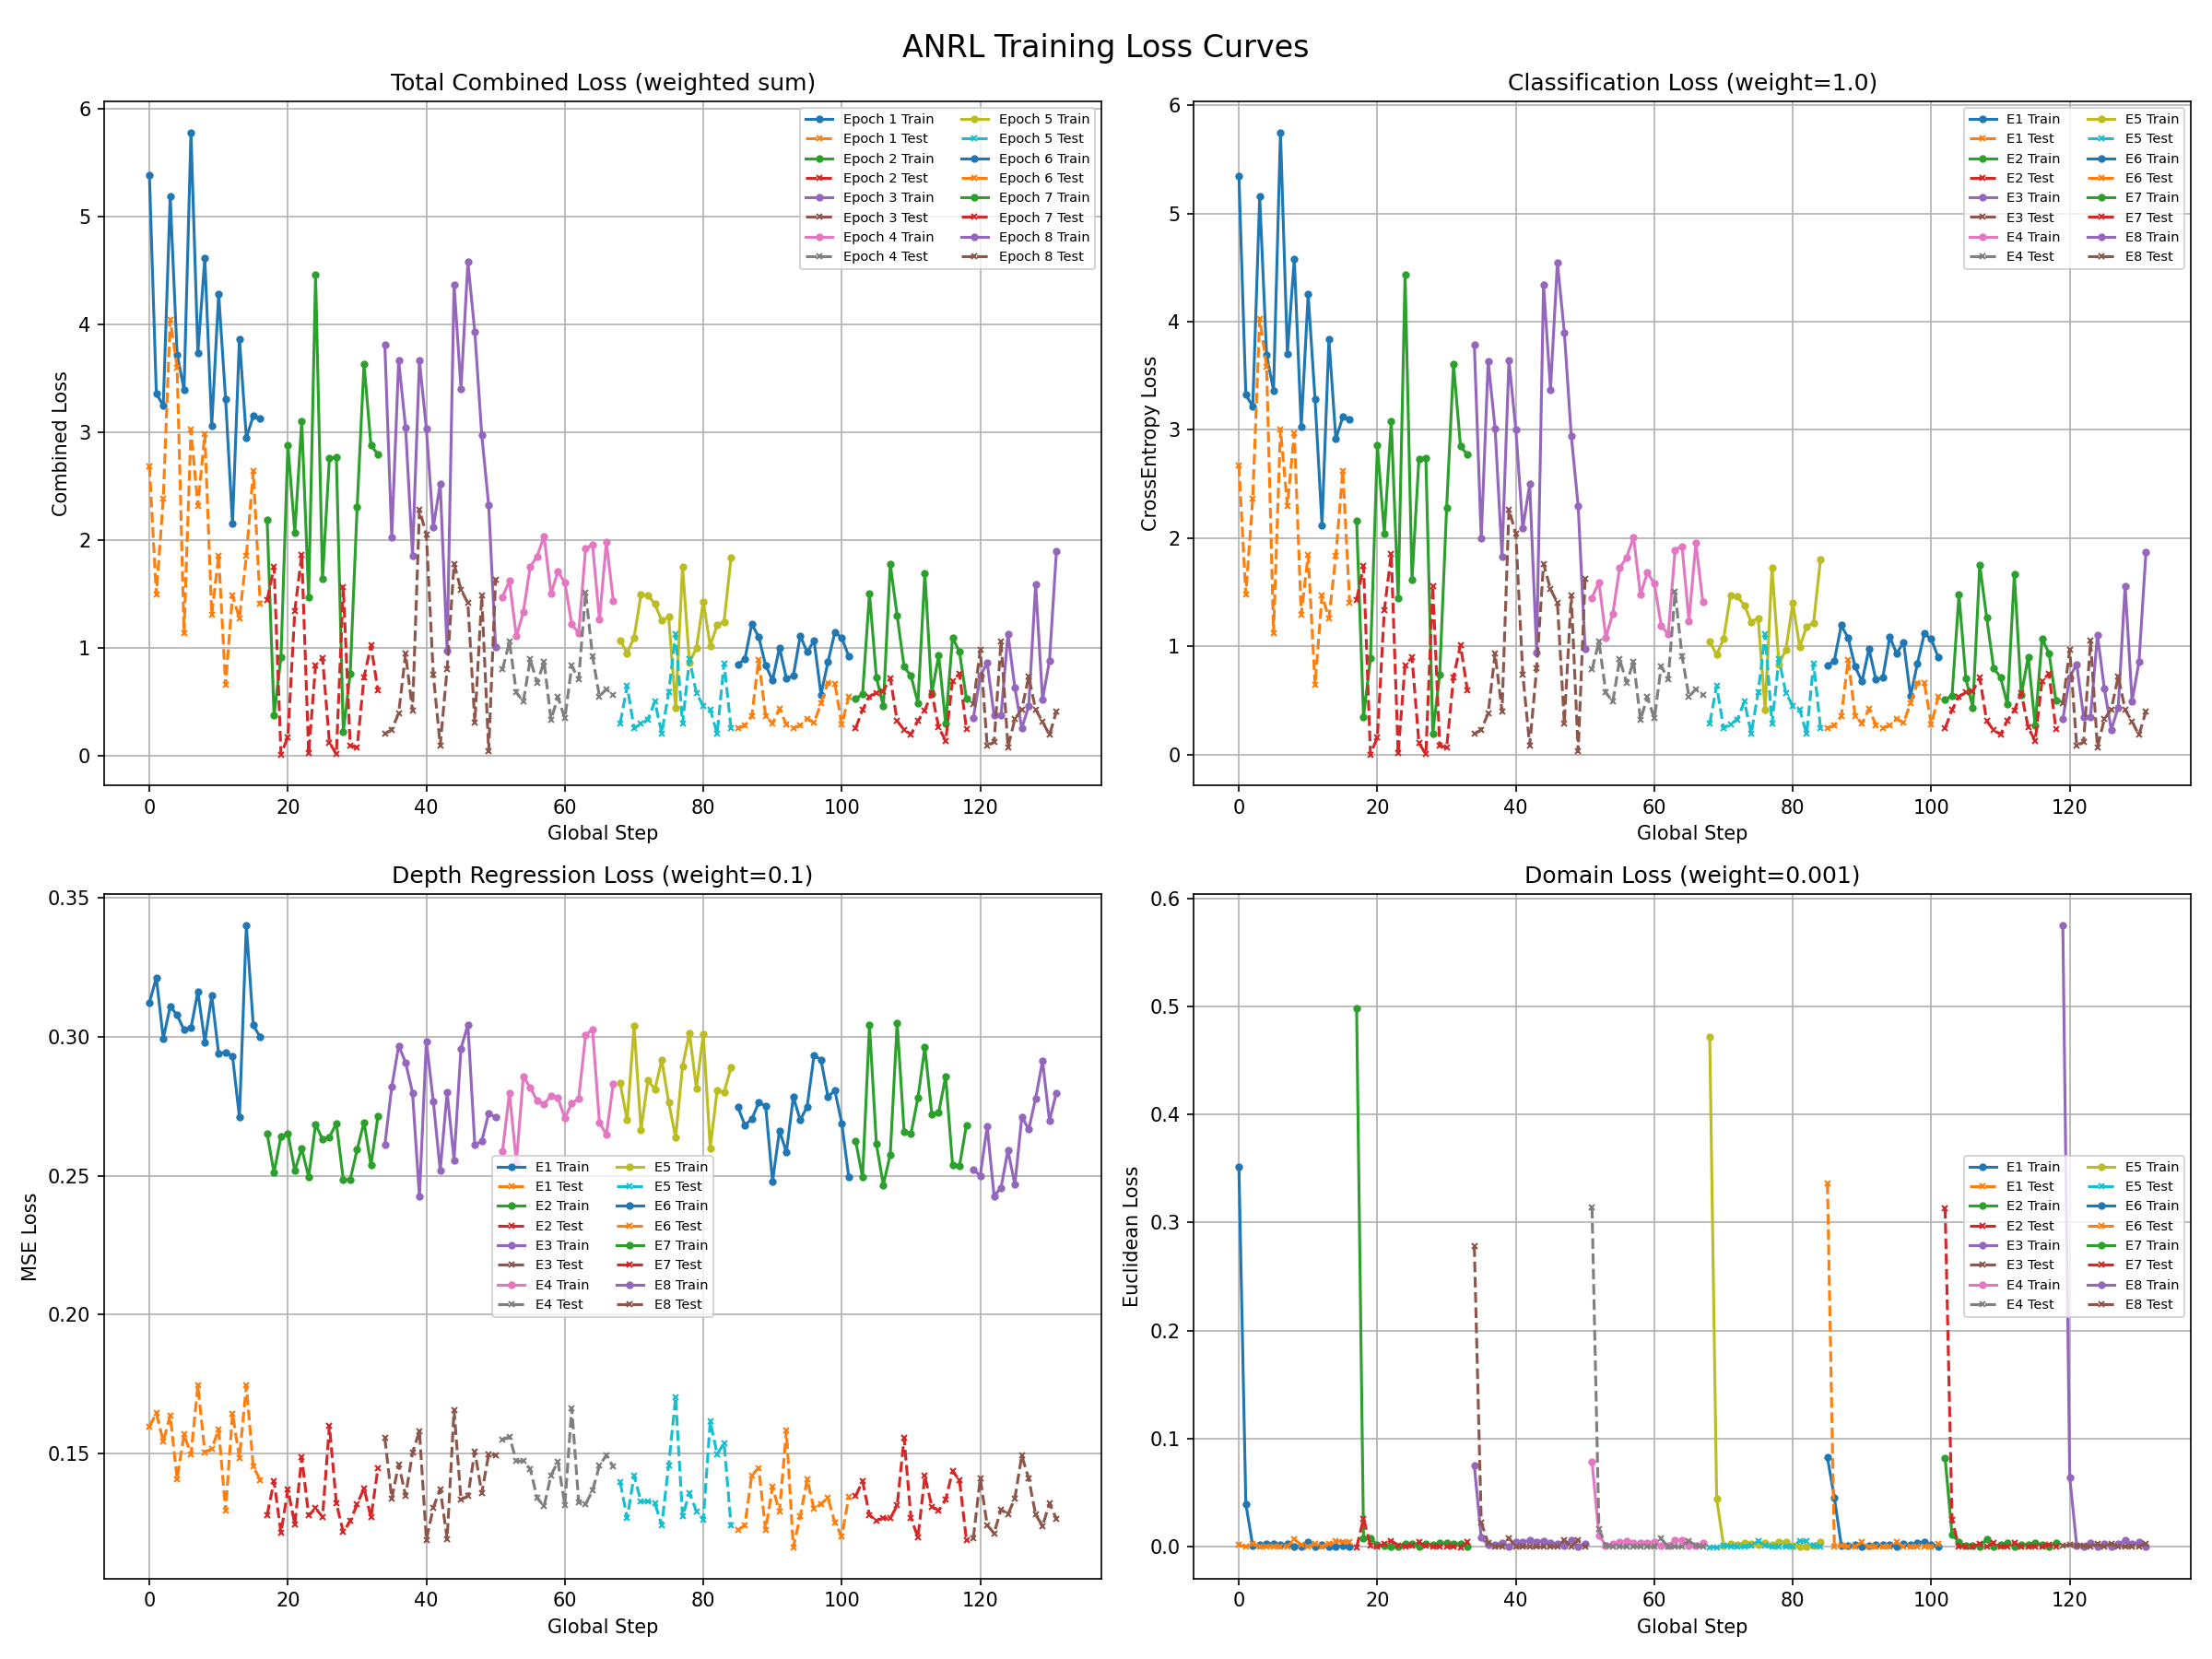
\includegraphics[width=\textwidth]{img/loss_curves.png}
            \caption{ANRL Training loss curves}
        \end{figure}
    \end{columns}
\end{frame}

% --- Slide 12: ANRL Framework Overview ---
\begin{frame}{ANRL Framework Architecture}
    \begin{figure}
        \centering
        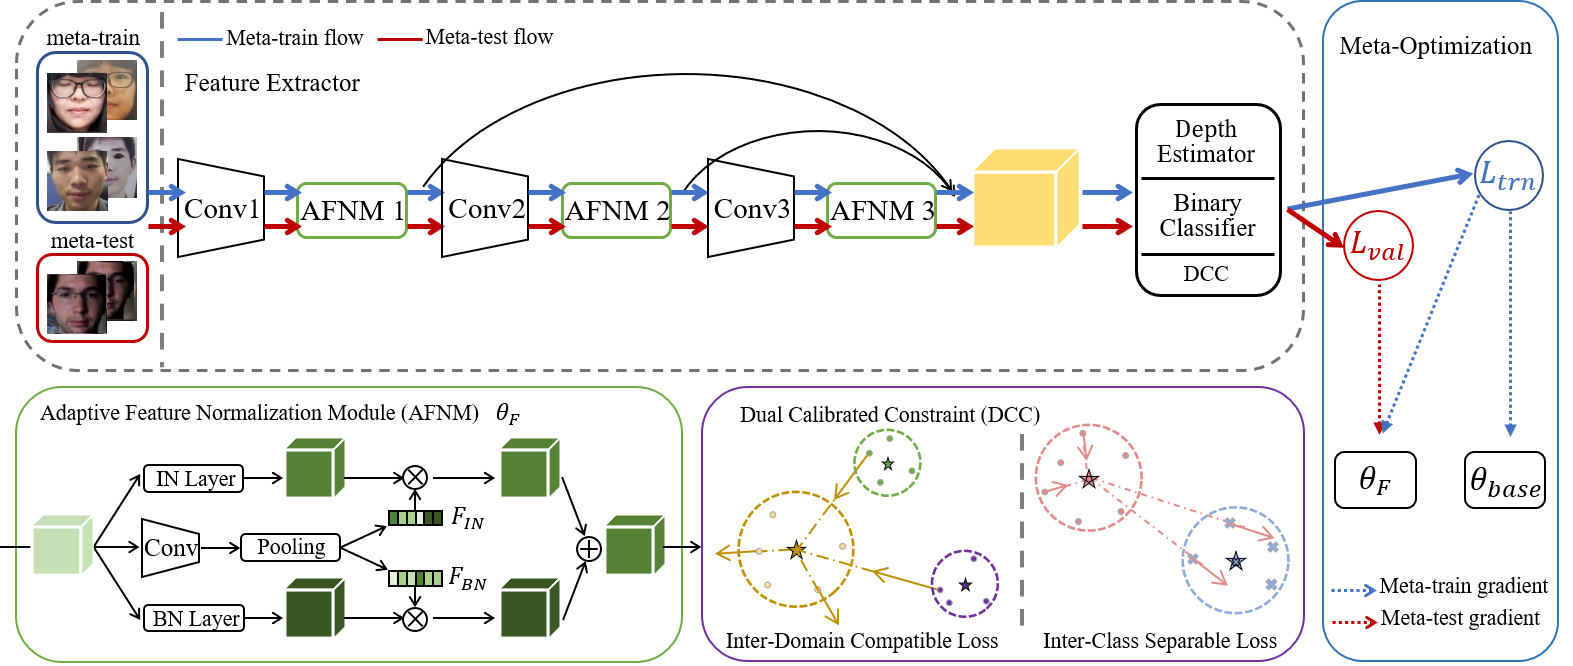
\includegraphics[width=0.85\textwidth]{img/framework.png}
        \caption{Overall ANRL Framework (Fig 2)}
    \end{figure}
    \vfill
    \begin{itemize}
        \item \textbf{CNN Backbone:} Located at the center as the shared \HL{Feature Extractor}.
        \item \textbf{Dual Pathways:} Integrates AFNM for both meta-train and meta-test episodes.
    \end{itemize}
\end{frame}

% --- Slide 13: Feature Extractor Specification ---
\begin{frame}{Technical Detail: Custom CNN Backbone}
    \centering
    \resizebox{0.8\textwidth}{!}{
    \begin{tabular}{@{}llcc@{}}
        \toprule
        \textbf{Stage} & \textbf{Layer} & \textbf{Channels/Stride} & \textbf{Output Size} \\ \midrule
        Input & Image & 6 (RGB+HSV) & 256 \\ \midrule
        Block 1 & conv1-1 to conv1-4 & 64--196 / 1 & 256 \\
        & pool1-1 & - / 2 & 128 \\ \midrule
        Block 2 & conv1-5 to conv1-7 & 128--196 / 1 & 128 \\
        & pool1-2 & - / 2 & 64 \\ \midrule
        Block 3 & conv1-8 to conv1-10 & 128--196 / 1 & 64 \\
        & pool1-3 & - / 2 & 32 \\ \bottomrule
    \end{tabular}
    }
    \vfill
    \begin{itemize}
        \item \textbf{Architecture:} 10-layer CNN backbone optimized for Colab T4 memory.
        \item \textbf{Note:} Connects directly to the \HL{Meta-Learner} and \HL{Depth Estimator} branches.
    \end{itemize}
\end{frame}

% --- Slide 14: Evaluation Protocol & Metrics ---
\begin{frame}{Evaluation Protocol \& Performance Metrics}
    \begin{block}{Primary Metrics}
        \begin{itemize}
            \item \textbf{AUC (Area Under Curve):} Evaluates the model's ability to rank real vs. spoof samples correctly across all thresholds.
            \item \textbf{HTER (Half Total Error Rate):} The average of False Rejection Rate (FRR) and False Acceptance Rate (FAR).
        \end{itemize}
    \end{block}

    \vfill
    \begin{itemize}
        \item \textbf{Goal:} Achieving \pos{Higher AUC} and \pos{Lower HTER} translates to better cross-domain generalization.
        \item \textbf{Note:} \HL{t-SNE} analysis is used to visualize feature separation between classes and domains.
    \end{itemize}
\end{frame}



\section{Source code implementation of core technical components}

% --- Slide 1: Section Title ---
\begin{frame}
    \vfill
    \centering
    \begin{beamercolorbox}[sep=8pt,center,shadow=true,rounded=true]{title}
        \usebeamerfont{title}Section 5.4: Source code implementation of core technical components [5]\par%
    \end{beamercolorbox}
    \vfill
\end{frame}

% --- Slide 2: Depth Map Supervision ---
\begin{frame}{1. Problem Definition \& Depth Supervision}
    \begin{block}{Geometric Depth Map Supervision [13]}
        \begin{itemize}
            \item \textbf{Rationale:} Forces the network to learn geometric structure (real faces are 3D) rather than relying on texture biases from 2D spoofs.
            \item \textbf{Code Identification:} \texttt{src/datasets/DG\_dataset.py} (Lines 60--62: setting depth to 0 for spoof labels).
            \item \textbf{Consequence:} Removing supervision leads to generalization failure; network "cheats" by focusing on high-frequency domain noise.
        \end{itemize}
    \end{block}
\end{frame}

% --- Slide 3: High-Dimensional Input ---
\begin{frame}{High-Dimensional Input Selection (RGB+HSV)}
    \begin{block}{Multi-Channel Rationale [2]}
        \begin{itemize}
            \item \textbf{Benefit:} HSV provides illumination (Value) and saturation signals robust to hardware-specific signatures.
            \item \textbf{Code Identification:} \texttt{src/datasets/DG\_dataset.py} (\texttt{img\_mode='rgb\_hsv'}).
            \item \textbf{Consequence:} RGB-only models increase vulnerability to brightness fluctuations [13], yielding higher \con{ACER/HTER} during cross-dataset testing.
        \end{itemize}
    \end{block}
\end{frame}

% --- Slide 4: AFNM Module Detail ---
\begin{frame}{2. AFNM: Adaptive Feature Normalization Module}
    \begin{block}{BN vs IN Trade-off [5]}
        \begin{itemize}
            \item \textbf{Rationale:} BN is discriminative but sensitive to domain gaps; IN is stable but discards FAS-relevant style info.
            \item \textbf{Code Identification:} \texttt{AttentionNet} in \texttt{src/models/base\_block.py} (Line 54).
            \item \textbf{Consequence:} Without AFNM, pure BN baseline HTER is \con{23.37\%} vs \pos{15.67\%} for ANRL (I\&C\&M $\to$ O task).
        \end{itemize}
    \end{block}
    \vfill
    \begin{itemize}
        \item \textbf{Principle:} Balance factor $\alpha_c$ per-sample: $Y_c = \alpha_c X_c^{BN} + (1-\alpha_c) X_c^{IN}$.
    \end{itemize}
\end{frame}

% --- Slide 5: DCC Constraints ---
\begin{frame}{3. DCC: Dual Calibrated Constraints}
    \begin{block}{IDC and ICS Loss Implementation}
        \begin{itemize}
            \item \textbf{Identification:} \texttt{src/train.py} (Lines 183--212). DCC uses exponential moving average (EMA) centroids (momentum 0.9).
            \item \textbf{Rationale:} IDC aligns domain representations; ICS increases inter-class separation.
            \item \textbf{Consequence:} Removing DCC results in an absolute \con{HTER increase of 2--4\%} (Table 3 in paper).
        \end{itemize}
    \end{block}
\end{frame}

% --- Slide 6: Meta-Learning training Flow ---
\begin{frame}{4. Meta-learning training Strategy}
    \begin{block}{Simulation of Domain Shift}
        \begin{itemize}
            \item \textbf{Steps:} 1. Inner Loop (Soft attention weights), 2. Meta-test, 3. Meta-Optimization.
            \item \textbf{Identification:} \texttt{src/train.py} (Lines 329--411). 
            \item \textbf{Rationale:} Enables AttentionNet to learn $\alpha$ estimation that generalizes to novel distributions.
            \item \textbf{Consequence:} HTER climbs from \pos{17.61\%} to \con{19.23\%} without meta-learning.
        \end{itemize}
    \end{block}
\end{frame}

% --- Slide 7: Network Architecture ---
\begin{frame}{5. Network Architecture}
    \begin{itemize}
        \item \textbf{FeatExtractor:} Integrates backbone with AFNM modules for domain-invariant extraction.
        \item \textbf{FeatEmbedder:} Discriminative head mapping features to class embeddings via ICS loss.
        \item \textbf{DepthEstimator:} Auxiliary head specialized in 3D geometric reconstruction.
    \end{itemize}
    \vfill
    \begin{block}{Architecture Selection Rationale}
        Modular framework decouples feature learning from classification and regression for stable shared learning.
    \end{block}
\end{frame}

% --- Slide 8: Paper to Code Mapping Summary ---
\begin{frame}{6. Summary: Paper $\leftrightarrow$ Code Mapping}
    \centering
    \resizebox{\textwidth}{!}{
    \begin{tabular}{@{}lll@{}}
        \toprule
        \textbf{Technique (Paper)} & \textbf{Code Component} & \textbf{Consequence of Removal} \\ \midrule
        Depth Supervision & \texttt{DepthEstimator} (MSE) & Overfitting to domain noise \\
        High-Dim Input & \texttt{rgb\_hsv} 6-ch & Low robustness to hardware [2] \\
        AFNM (BN+IN) & \texttt{AdapNorm} Logic & HTER increase \con{+7.7\%} \\
        DCC Losses & \texttt{loss\_domain}, \texttt{loss\_discri} & Loss of domain alignment \\
        Meta-learning & \texttt{train()} Outer Loop & Higher HTER \con{+1.62\%} \\ \bottomrule
    \end{tabular}
    }
\end{frame}



% % Slide 4: Paper Methodology
% \input{section/02_methodology.tex}

% % Slide 5: Relationship of book and paper
% \input{section/03_relationship.tex}

% % Slide 6: Technical evaluation
% \input{section/04_evaluation.tex}

% % Slide 7: Insights & Extensibility
% % 5. Personal technical insights and extensibility
\section{Personal insights: extensibility}

\begin{frame}[fragile]{Future extensibility}
    \textbf{Extension 1: Simulating Spoofing Clues (Augmentation) \cite{he2024joint}.} \\
    To overcome reliance on diverse source domains, ANRL can be extended with Joint Physical-Digital augmentation. During Meta-Train, live faces are augmented into simulated attacks ($X_{sim}$) using Simulated Physical (e.g., color distortion, $\theta_{SPSC}$) and Digital (e.g., Gaussian blur, $\theta_{SDSC}$) Spoofing Clues.
    \begin{equation}
        X_{sim} = Aug(X_{real}; \theta_{SPSC}, \theta_{SDSC})
    \end{equation}
    
    \begin{figure}[ht]
    \centering
    \scalebox{0.55}{
    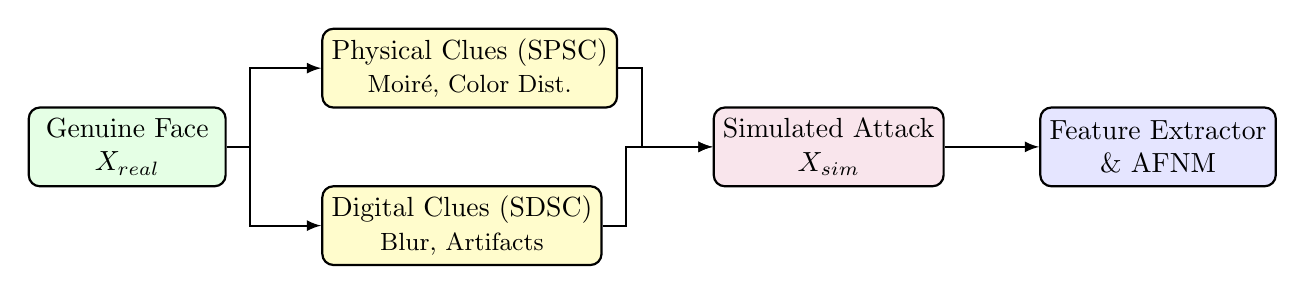
\begin{tikzpicture}[
        >=latex,
        node distance=1.0cm and 1.2cm,
        box/.style={draw, rectangle, rounded corners, thick, align=center, fill=blue!10, minimum height=1cm, minimum width=2.5cm},
        augbox/.style={draw, rectangle, rounded corners, thick, align=center, fill=yellow!20, minimum height=1cm, minimum width=2.5cm},
        arrow/.style={->, thick}
    ]
    % Nodes
    \node[box, fill=green!10] (input) {Genuine Face \\ $X_{real}$};
    \node[augbox, right=of input, yshift=1cm] (spsc) {Physical Clues (SPSC) \\ \small Moir\'e, Color Dist.};
    \node[augbox, right=of input, yshift=-1cm] (sdsc) {Digital Clues (SDSC) \\ \small Blur, Artifacts};
    \node[box, fill=purple!10, right=of spsc, yshift=-1cm] (xsim) {Simulated Attack \\ $X_{sim}$};
    \node[box, right=of xsim] (afnm) {Feature Extractor \\ \& AFNM};

    % Arrows
    \draw[arrow] (input.east) -- ++(0.3,0) |- (spsc.west);
    \draw[arrow] (input.east) -- ++(0.3,0) |- (sdsc.west);
    \draw[arrow] (spsc.east) -| ++(0.3,-1) -- (xsim.west);
    \draw[arrow] (sdsc.east) -| ++(0.3, 1) -- (xsim.west);
    \draw[arrow] (xsim.east) -- (afnm.west);
    \end{tikzpicture}
    }
    \end{figure}
\end{frame}

\begin{frame}{Future extensibility (cont.)}
    \textbf{Extension 2: Temporal-Spectral ANRL (TS-ANRL).} \\
    While ANRL excels in 2D spatial generalization, practical FAS heavily relies on temporal cues (e.g., eye blinking). Extending AFNM with 3D convolutions allows temporal-IN to filter dynamic lighting fluctuations, while temporal-BN preserves chronological inconsistencies inherent to video replay attacks.
\end{frame}


% % Slide 8: References
% \input{section/06_references.tex}

\end{document}
